\section[تمرین اول - سؤال چهارم: خوشه‌بندی ترکیبی گوسی (GMM)]
{\faProjectDiagram\ \ تمرین اول ـ سؤال چهارم: خوشه‌بندی نرم داده‌ها با مدل ترکیبی گوسی (\lr{GMM})}

\begin{stepbox}

\field{هدف و معرفی مسئله}{
هدف این بخش، پیاده‌سازی و بررسی الگوریتم **مدل ترکیبی گوسی (\lr{Gaussian Mixture Model - GMM})** و مقایسه مفاهیم خوشه‌بندی سخت (\lr{Hard Clustering}) مانند \lr{K-Means} با خوشه‌بندی نرم (\lr{Soft Clustering}) می‌باشد.

در الگوریتم‌های خوشه‌بندی نرم، هر نمونه برعکس الگوریتم‌های معمولی به صورت قطعی به یک خوشه متصل نمی‌شود، بلکه یک توزیع احتمالی از میزان تعلق نقطه به هر یک از توابع گوسی (خوشه‌ها) محاسبه می‌گردد. مجموعه داده مورد استفاده در این تمرین شامل ۴۰۰ نمونه دوبعدی تولیدشده توسط تابع \lr{make\_blobs} است.
}

\field{ارزیابی اولیه و خوشه‌بندی با K-Means}{
با بررسی نمودار پراکندگی اولیه داده‌ها، وجود ۴ مرکز توزیع واضح در فضای داده مشاهده گردید. در مرحله نخست، الگوریتم \lr{K-Means} با انتخاب $k=4$ اجرا گردید.

الگوریتم \lr{K-Means} با فرض کروی بودن مرز خوشه‌ها و تخصیص قطعی مرزها عمل می‌کند. نتایج این خوشه‌بندی در شکل زیر آورده شده است.

\vspace{0.4cm}

\begin{center}
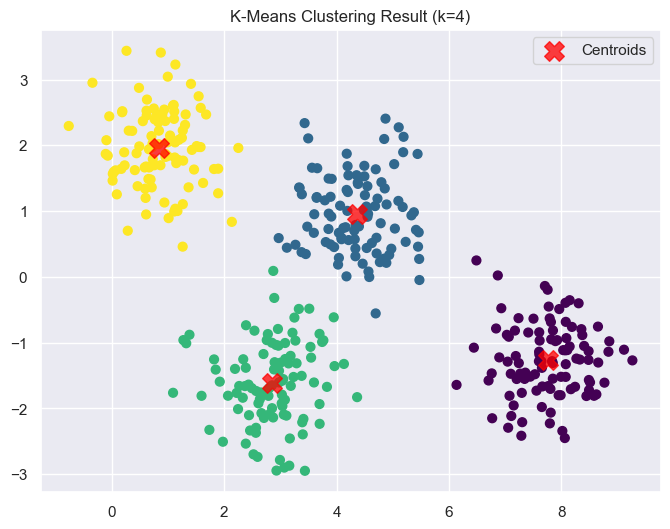
\includegraphics[width=.70\textwidth]{images/kmeans_gmm_comparison.png}
\captionof{figure}{نتیجه خوشه‌بندی داده‌ها توسط الگوریتم \lr{K-Means} ($k=4$)}
\label{fig:kmeans_gmm}
\end{center}
}

\field{آموزش مدل GMM و محاسبه ماتریس احتمالات}{
در ادامه، مدل \lr{GaussianMixture} از ماژول \lr{sklearn.mixture} با تعیین $n\_components=4$ روی داده‌ها برازش داده شد. سپس با استفاده از متد \lr{predict\_proba}، ماتریس احتمالات به ابعاد $(400, 4)$ محاسبه گردید.

هر سطر از این ماتریس، احتمال حضور یک نمونه داده را در ۴ تابع توزیع گوسی نشان می‌دهد. جهت ملموس‌تر شدن مفهوم عدم قطعیت (\lr{Uncertainty})، اندازه نقاط در نمودار متناسب با حداکثر احتمال تعلق آن‌ها تنظیک گردید:

\vspace{0.4cm}

\begin{center}
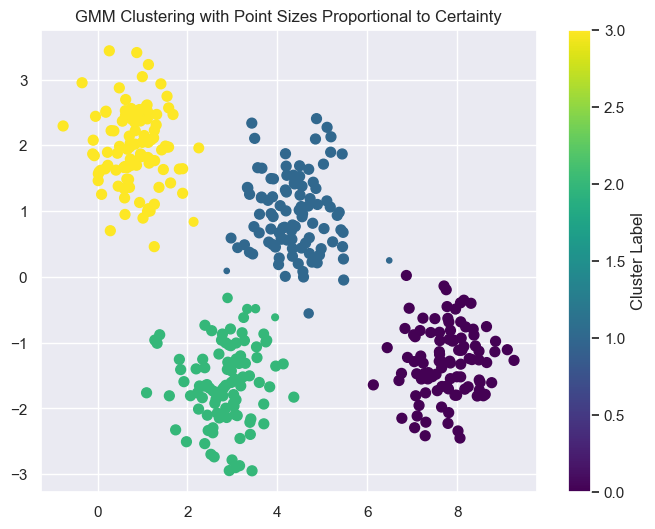
\includegraphics[width=.72\textwidth]{images/gmm_uncertainty_plot.png}
\captionof{figure}{نمایش میزان قطعیت خوشه‌بندی نمونه‌ها (اندازه بزرگتر نشان‌دهنده احتمال تعلق بالا به خوشه است)}
\label{fig:gmm_prob}
\end{center}
}

\field{رسم بیضی‌های کواریانس و تحلیل خروجی}{
با تکمیل توابع \lr{draw\_ellipse} و \lr{plot\_gmm}، بیضی‌های هم‌احتمال توزیع‌های گوسی برای هر خوشه ترسیم شدند. این بیضی‌ها ماتریس کواریانس و نحوه پراکندگی داده‌های هر خوشه را نمایش می‌دهند.

\vspace{0.4cm}

\begin{center}
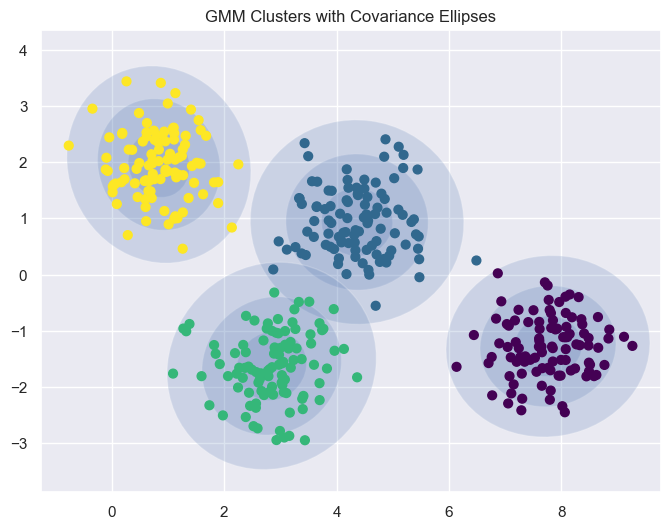
\includegraphics[width=.75\textwidth]{images/gmm_ellipses_result.png}
\captionof{figure}{نتیجه خوشه‌بندی \lr{GMM} به همراه بیضی‌های توزیع کواریانس خوشه‌ها}
\label{fig:gmm_ellipses}
\end{center}
}

\field{نتایج و استنباط تحلیلی}{
تحلیل و استنباط حاصل از خروجی‌های مدل \lr{GMM}:

\begin{itemize}
\item **خوشه‌بندی نرم در برابر سخت:** برعکس \lr{K-Means} که نقاط مرزی را مجبورا به یک خوشه نسبت می‌دهد، \lr{GMM} عدم قطعیت نقاط مرزی را بر حسب احتمال بازگو می‌کند.
\item **شکل خوشه‌ها:** استفاده از ماتریس کواریانس عمومی به \lr{GMM} این امکان را می‌دهد تا خوشه‌های بیضوی و کشیده را نیز بهتر از \lr{K-Means} پوشش دهد.
\item **میزان انحراف:** بیضی‌های مرکز خوشه‌ها فشرده‌تر و بیضی‌های بیرونی نشان‌دهنده انحراف معیار‌های بالاتر ($\sigma, 2\sigma, 3\sigma$) در توزیع گوسی متناظر هستند.
\end{itemize}
}

\field{جمع‌بندی}{
در این بخش، الگوریتم \lr{GMM} با ۴ مؤلفه گوسی پیاده‌سازی و ارزیابی شد. نتایج نشان داد که این الگوریتم به‌واسطه ارائه خروجی احتمالی (\lr{predict\_proba}) و انعطاف‌پذیری هندسی به کمک ماتریس کواریانس، ابزاری بسیار قدرتمندتر نسبت به \lr{K-Means} برای تحلیل داده‌هایی با مرزهای مبهم یا توزیع‌های بیضوی است.
}

\end{stepbox}